\chapter{Cosmologia di Friedmann-Lema\^itre-Robertson-Walker}\label{para.cosmo}
La cosmologia ha come scopo la descrizione dell'universo nel suo insieme, cercando di spiegarne l'origine e l'evoluzione. Scopo di questa sezione è determinare quali soluzioni alle equazioni di Einstein sono idonee alla descrizione dell'universo e sotto quali ipotesi avvengono. Verrà fatta un'overview generale degli aspetti fondamentali legati alla cosmologia FLRW, per la descrizione di un universo omogeneo e isotropo.

\section{Omogeneità e isotropia}
All'interno del modello cosmologico si assumono le ipotesi che esso sia \emph{omogeneo} e \emph{isotopo}. Da un punto di vista storico già dagli studi di Copernico si è consolidata l'idea che la posizione nell'universo non fosse privilegiata. Se ci trovassimo in un'altra regione dell'universo le caratteristiche di base del nostro intorno sarebbero le stesse. Un universo omogeneo è un universo indipendente dalla posizione.

Similmente non ha senso assumere che esistano direzioni privilegiate, da cui l'ipotesi dell'isotropia. \'E importante osservare che queste ipotesi di carattere filosofico sono comunque supportate sperimentalmente: in particolare su grandi scale si è osservato che la distribuzione delle galassie è isotropa e omogenea (nonostante a scale minori si possano osservare \emph{clusters} di galassie e regioni prive di esse) ed inoltre gli studi sulla radiazione cosmica di fondo (CMB) hanno riportato analoghi risultati.

Esprimiamo rigorosamente l'omogeneità e l'isotropia:
\begin{definizione}
Uno spaziotempo $\mathcal{M}$ è (spazialmente) \textbf{omogeneo} se esiste una famiglia ad un parametro di ipersuperfici $\Sigma_t$ di tipo spazio tali che
\begin{equation*}
    \bigcup_t \Sigma_t = \mathcal{M}
\end{equation*}
e $\forall t$, $\forall p,q \in \Sigma_t$ esiste sempre un'isometria $f$ della metrica $g_{\mu\nu}$ tale che $f(p)=q$ cioè che mappa uno nell'altro.
\end{definizione}

\begin{definizione}
Uno spaziotempo $\mathcal{M}$ è (spazialmente) \textbf{isotropo} in ogni punto se esiste una congruenza di curve di tipo tempo con vettori tangenti $u$ tali che:
\begin{enumerate}
    \item Lo spaziotempo $\mathcal{M}$ è unione delle curve.
    \item Dato $p$ qualsiasi e due vettori $s_1, s_2 \perp u$ in $p$, esiste sempre un'isometria che lascia $p,u$ invariati e ruota $s_1$ in $s_2$.
\end{enumerate}
\end{definizione}

Quest'ultimo punto è quello che permette di dire che non ci sono vettori spaziali preferiti ovvero che non si può costruire vettore perpendicolare a $u$ che sia geometricamente privilegiato.

Come conseguenza di queste definizioni, in un universo omogeneo e isotropo le ipersuperfici $\Sigma_t$ devono essere perpendicolari ai vettori tangenti $u$, altrimenti proiettando quest'ultimo sull'ipersuperficie si potrebbe costruire un vettore geometricamente preferito.

Con queste considerazioni si ha che la metrica $g_{\mu\nu}$ induce sulla ipersuperficie (3-dimensionale) $\Sigma_t$ una metrica $h_{\mu\nu}(t)$ (vale a dire restringere $g$ ai vettori tangenti alla superficie).
\begin{align*}
    g_{\mu\nu} = -u_\mu u_\nu +h_{\mu\nu}(t)  \overset{\cdot u^\nu}{\longrightarrow} g_{\mu\nu} u^\nu &= -u_\mu u_\nu u^\nu + h_{\mu\nu}(t)u^\nu \\
     u_\mu &= u_\mu + h_{\mu\nu}(t)u^\nu
\end{align*}
ciò implica $ h_{\mu\nu} u^\nu = 0$ (proiettore) e che $u$ sia autovettore di $h$ con autovalore nullo. Segue che possiamo esprimere la matrice di $h$ almeno nella forma:
\begin{equation*}
    h_{\mu\nu}(t) =
  \begin{pmatrix}
  0 & 0 & 0& 0 \\
  0& & & & \\
  0& &   h_{ij}(t)& & \\
  0& & & &
  \end{pmatrix}
\end{equation*}

cioè isolando in un blocco tale autovalore, e lasciando indeterminata la restante matrice 3x3. Vediamo ora quali conseguenze su $h_{ij}$ comportano l'omogeneità e l'isotropia.

Consideriamo il tensore di Riemann costruito sulla metrica $h_{ij}$: $\tensor{R}{^i_{jkl}}$. Questo viene alzato da $h$ in $\tensor{R}{^{ij}_{kl}}$ antisimmetrico nello scambio delle coppie $ij$, $kl$ per via delle proprietà generali del tensore. Pertanto si ha l'applicazione lineare:
\begin{align*}
    L : W &\rightarrow W \\
    \omega_{ij} &\mapsto \tilde{\omega}_{kl} =\tensor{R}{^{ij}_{kl}}\omega_{ij}
\end{align*}
dove $W$ è lo spazio vettoriale delle 2-forme. Poiché $\tensor{R}{^{ij}_{kl}} = \tensor{R}{_{kl}^{ij}}$ sempre per le proprietà del tensore, allora l'applicazione $L$ è simmetrica e pertanto ammette base ortonormale di autovettori.

Per l'ipotesi sulla isotropia, tutti gli autovalori di L devono essere uguali e quindi $L$ risulta multiplo dell'identità:
\begin{equation*}
    L = k \mathds{1}
\end{equation*}
Infatti se così non fosse, supponiamo si abbiano gli autovalori $\lambda_1, \lambda_2 = \lambda_3$, si avrebbe per il primo l'autovettore $\omega^{(1)}_{ij}$ che determina il vettore spaziale $v^k = \epsilon^{ijk}\omega^{(1)}_{ij}$. Questo sarebbe un vettore spaziale preferito e quindi contro l'isotropia.

L'omogeneità implica invece che $k$ non dipenda dalla posizione, ma al massimo dal tempo. Si ottiene quindi il tensore di Riemann (di dim. 3) costruito sulla metrica indotta sulle ipersuperfici di tipo spazio $\Sigma_t$:
\begin{equation}
    \tensor{R}{^{ij}_{kl}} = k \tensor{\delta}{^i_{[k}} \tensor{\delta}{^j_{l]}}
    \label{eq.R_curva_cost}
\end{equation}
L'antisimmetrizzazione sugli indici delle $\delta$ è inserita per mantenere l'antisimmetria del tensore a sinistra.

Osserviamo che $k= \textrm{cost.}$ segue anche dalla seconda identità di Bianchi: $\tensor{R}{^{ij}_{[jk;m]}}=0$. Esplicitamente su \cite{wald}. Questo comporta che si potrebbe fare anche a meno dell'ipotesi sull'omogeneità, ma è anche da osservare che la richiesta di isotropia in ogni punto implica essa stessa l'omogeneità.

\begin{definizione}
Uno  spaziotempo $\mathcal{M}$ che soddisfa eq. \ref{eq.R_curva_cost} si dice \textbf{a curvatura costante}.
\end{definizione}

Mostriamo che per uno spazio a curvatura costante vale eq. \ref{eq.riemann_curvatura_costante}. Il calcolo è abbastanza diretto, dovendo soltanto abbassare i primi due indici:
\begin{equation*}
    R_{\mu\nu\rho\sigma} = g_{\mu\alpha}g_{\nu\beta} \tensor{R}{^{\alpha\beta}_{\rho\sigma}} = kg_{\mu\alpha}g_{\nu\beta}(\tensor{\delta}{^\alpha_\rho}\tensor{\delta}{^\beta_\sigma} - \tensor{\delta}{^\alpha_\sigma}\tensor{\delta}{^\beta_\rho}) = k(g_{\mu\rho}g_{\nu\sigma} - g_{\mu\sigma}g_{\nu\rho})
\end{equation*}

Facciamo vedere inoltre che per tale spazio si può esprimere $k$ in funzione dello scalare di Ricci secondo eq. \ref{eq.costvettorikillinglambda}. Per fare questo ricordiamo che la traccia dell'identità è pari alla dimensione dello spazio, ovvero $\tensor{\delta}{^\sigma_\sigma} = n$. Calcoliamo il Ricci da eq. \ref{eq.R_curva_cost}:
\begin{align*}
    \tensor{R}{^\nu_\sigma} &= \tensor{R}{^{\mu\nu}_{\mu\sigma}} = k(\tensor{\delta}{^\mu_\mu}\tensor{\delta}{^\nu_\sigma} - \tensor{\delta}{^\mu_\sigma}\tensor{\delta}{^\nu_\mu}) \\
    &= k(n\tensor{\delta}{^\nu_\sigma} - \tensor{\delta}{^\mu_\sigma}\tensor{\delta}{^\nu_\mu}) =k(n-1)\tensor{\delta}{^\nu_\sigma}
\end{align*}
Quindi lo scalare di Ricci:
\begin{equation*}
    R = \tensor{R}{^\sigma_\sigma} = k(n-1)\tensor{\delta}{^\sigma_\sigma} = k n(n-1)
\end{equation*}

Poiché l'ipersuperficie di omogeneità $\Sigma_t$ è di dimensione 3, si avrà che $R=6k$.
\section{Metrica FLRW}

Si deve a Luther P. Eisenhart nel 1949 la classificazione degli spazi a curvatura costante di dimensione $n$ e con segnatura $n$ (quindi tutti autovalori positivi della metrica). Tali spazi sono isometrici a:
\begin{itemize}
    \item $H^n$ spazio iperbolico se $k<0$.
    \item $\mathbb{E}^n$ spazio euclideo se $k=0$.
    \item $S^n$ $n$-sfera se $k>0$.
\end{itemize}
La geometria spaziale dell'universo è una di queste tre. Nella fisica prerelativistica, così come nella relatività ristretta, si assume uno spazio piatto, $k=0$; è interessante notare come le richieste più restringenti di omogeneità e isotropia permettano di avere ulteriori due possibilità.

Aspetto fondamentale dello spazio $S^n$ è che descrive un universo chiuso, cioè finito, ma senza bordo (un palloncino è finito, ma non ha un bordo), mentre lo spazio piatto e iperbolico sono aperti.

La metrica di $S^3$ è:
\begin{equation}
    ds^2 = l^2(d\psi^2 +\sin^2\psi( d\theta^2 + \sin^2\theta d\phi^2))
    \label{eq.metrica_s3}
\end{equation}
definendo il termine tra parentesi $(d\Omega_1)^2$. Il pedice corrisponde a $k=1$. Questa può essere ricavata considerando l'embedding in $\mathbb{E}^4$ dotato di metrica $ds^2 = dx^2+ dy^2 + dz^2 + dw^2$. L'ipersuperficie corrisponde a:
\begin{equation*}
    x^2 + y^2 + z^2 + w^2 = l^2
\end{equation*}
dove se introduciamo la coordinata $w = l\cos\psi$, si ottiene:
\begin{equation*}
    x^2 + y^2 + z^2 = l^2\sin^2\psi
\end{equation*}
pari ad una sfera di raggio $l\sin\psi$\footnote{Si può infatti immaginare la 3-sfera come una sfera che cambia raggio al variare della distanza dal centro.}. Esprimendo le restanti coordinate con le coordinate sferiche usuali si ottiene la metrica eq. \ref{eq.metrica_s3}.

La metrica di $H^3$ é:
\begin{equation}
    ds^2 = l^2(d\psi^2 +\sinh^2\psi( d\theta^2 + \sin^2\theta d\phi^2))
    \label{eq.metrica_h3}
\end{equation}
definendo il termine tra parentesi $(d\Omega_{-1})^2$, con $k=-1$. Questa si ottiene considerando l'embedding in $\mathbb{M}^4$ dotato di metrica $ds^2 =-dt^2 + dx^2 +dy^2 +dz^2$. L'ipersuperficie corrisponde a:
\begin{equation*}
    t^2 - x^2 - y^2 -z^2 = l^2
\end{equation*}
dove se introduciamo la coordinata $t = l\cosh\psi$, si ottiene:
\begin{equation*}
    x^2 + y^2 + z^2 = l^2\sinh^2\psi
\end{equation*}
pari ad una sfera di raggio $l\sinh\psi$. Anche qui le restanti coordinate vengono espresse con le usuali sferiche per ricavare eq. \ref{eq.metrica_h3}.

La metrica di $\mathbb{E}^3$ è la nota in coordinate polari:
\begin{equation}
    ds^2 = d\psi^2 + \psi^2(d\theta^2 +\sin^2\theta d\phi^2)
\end{equation}
definendola $(d\Omega_0)^2$. 

Alla luce di quanto detto, in 4 dimensioni si sceglierà un sistema di coordinate iperbolico, sferico o cartesiano in base al valore di $k$ e queste coordinate verranno portate sulla ipersuperficie di omogeneità $\Sigma_t$.
Dunque tramite gli \textbf{osservatori isotropi}, cioè osservatori con vettore tangente $u$, si portano tali coordinate su tutte le altre ipersuperfici. In altri termini ogni osservatore isotropo ha delle coordinate spaziali fisse e il parametro $\tau$ del tempo proprio (misurato dall'orologio di questi osservatori isotropi) diventa un'ottima coordinata per etichettare ogni ipersuperficie. Pertanto il tempo proprio e le coordinate spaziali permettono di individuare ogni evento nell'universo, fig. \ref{fig.osservatori_iso}.
Per l'omogeneità tutti gli osservatori isotropi misurano la stessa differenza di tempo proprio tra due ipersuperfici.
\begin{figure}
    \centering
    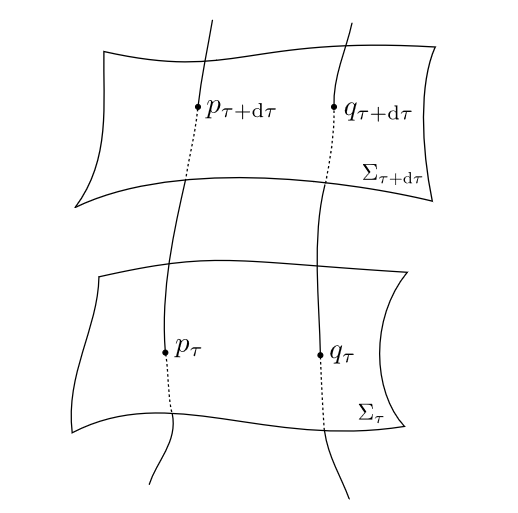
\includegraphics[scale=0.5]{immagini/osservatori_isotropi.png}
    \caption{Il tempo proprio permette di identificare le ipersuperfici di omogeneità. La differenza di tempo proprio misurata tra le due ipersuperfici dai due osservatori è la stessa.}
    \label{fig.osservatori_iso}
\end{figure}
La metrica in 4 dimensioni é:
\begin{equation}
    ds^2 = -d\tau^2 + a^2(\tau)d\Omega_k^2
    \label{eq.metrica_flrw}
\end{equation}
che viene detta \textbf{metrica di Friedmann-Lema\^itre-Robertson-Walker}, dove $k=0,\pm 1$ e $a(\tau)$ fattore di scala o anche detto parametro di scala dell'universo. L'elemento $d\Omega_k$ rappresenta lo spostamento sulla sottovarietà omogenea e isotropa tridimensionale. Si osserva che i termini $l$ che appaiono in eq. \ref{eq.metrica_s3}, \ref{eq.metrica_h3} sono assorbiti dal fattore $a$.
Questo non è determinato da ipotesi di simmetria come il resto della metrica, ma deve essere determinato inserendo la metrica nelle equazioni di Einstein eq. \ref{eq.GRequazioneeinstein}. Ovviamente in queste manca un aspetto che non si è ancora affrontato, ovvero quale sia il tensore di energia-impulso idoneo a descrivere l'universo.

\section{Galassie, polveri, radiazione ed energia oscura}\label{para.polveri}
Il primo elemento che va incluso per la descrizione dell'universo è la materia ordinaria e in particolare le galassie composte da essa. Le galassie possiamo assimilarle con buona approssimazione ad un \textbf{polvere} nel contesto cosmologico in quanto ciò può essere supportato da misure cosmiche. Con polvere si intende che questi elementi di materia ordinaria non possiedono pressione, $P=0$; le velocità casuali delle galassie sono piccole e ciò permette di trascurare la pressione di questa polvere di galassie.
All'interno di questo modello, il fluido cosmico sarà quindi idealizzato in un fluido perfetto, già descritto in \S\ref{para.fluido}:
\begin{equation*}
    T_{\mu\nu} = \rho u_\mu u_\nu
\end{equation*}
dove $\rho$ è la densità di massa media della materia e $u$ è il vettore tangente alle linee di mondo. Osserviamo infatti che le linee di mondo delle galassie devono coincidere con quelle degli osservatori isotropi in quanto il moto relativo tra questi può essere usato come direzione privilegiata. Proprio per via di questo moto relativo trascurabile, possiamo adottare come tensore energia-impulso quello del fluido perfetto relativistico.

Oltre alla materia ordinaria si considera anche la presenza della radiazione elettromagnetica con tensore energia-impulso:
\begin{equation*}
    T_{\mu\nu} = \frac{1}{4\pi} \left[ F_{\mu\alpha}\tensor{F}{^\alpha_\nu} - \frac{1}{4}g_{\mu\nu}F_{\alpha\beta}F^{\alpha\beta} \right]
\end{equation*}
è tensore a traccia nulla, $\tensor{T}{^\mu_\mu}=0$. Usando l'eq. \ref{eq.fluidoperfetto} del fluido perfetto e ponendo la traccia nulla, si ottiene l'equazione di stato per la radiazione:
\begin{equation*}
    P = \frac{\rho}{3}
\end{equation*}

L'energia-impulso nella forma di fluido perfetto che ci permette di descrivere l'universo è la fusione delle due ed è la forma più generale e compatibile con l'omogeneità e isotropia.
\begin{equation*}
    T_{\mu\nu} = \rho u_\mu u_\nu + P(g_{\mu\nu} +u_\mu u_\nu)
\end{equation*}

Normalmente ci si sarebbe fermati qui: considerata la radiazione e la materia ordinaria non ci dovrebbe essere null'altro. Purtroppo non è proprio così. Grazie ai loro lavori del 1998 \cite{1998_1} \cite{1998_2}, Saul Perlmutter, Brian P. Schmidt e Adam G. Riess (premi Nobel nel 2011), mostrarono attraverso l'osservazione del redshift di supernove l'espansione dell'universo e che questo stesse pure accelerando. Ulteriori osservazioni delle anisotropie della CMB, delle abbondanze degli elementi dovute alla nucleosintesi primordiale (elio in particolare), della struttura a grande scala dell'Universo, del clustering di galassie e delle misurazioni del parametro di Hubble hanno confermato l'espansione dell'universo nonché forniscono un importante confronto tra la teoria e le osservazioni. Il modello attualmente più soddisfacente per spiegare queste osservazioni prende il nome di $\Lambda$CDM (\emph{cold dark matter}). Chiaramente qui si vedrà la descrizione base.

Si è quindi introdotto il concetto di \textbf{energia oscura} per giustificare l'esistenza di una forza \emph{antigravitazionale} che giustificasse questa rapida espansione. Dagli studi sulla CMB, in particolare per mezzo del satellite WMAP, si è potuto stimare che l'universo fosse composto approssimativamente  da $\sim 5\%$ da materia ordinaria (barionica), $\sim 22\%$ da materia oscura (materia di natura sconosciuta, non osservabile tramite radiazione) e per il $\sim 73 \%$ da energia oscura. Questa energia oscura potrebbe essere rappresentata dalla \textbf{energia del vuoto}, concetto emerso dalla teoria quantistica dei campi che descrive l'energia dovuta alle cosiddette \emph{fluttuazioni del vuoto} ovvero alla continua annichilazione di coppie particella-antiparticella virtuali.

Il più semplice modello di energia oscura che tratteremo qui sarà basato sulla \textbf{costante cosmologica} $\Lambda$. Un aspetto fondamentale è che questa densità di energia associata alla costante è incredibilmente piccola per gli standard della fisica delle particelle; ciò rende complicato il legame con l'energia del vuoto, visto che tutti questi contributi energetici dovrebbero partecipare all'effettivo valore della costante. La natura dell'energia oscura, il suo legame con le altre branche della fisica e il valore della costante $\Lambda$ sono tutti problemi ancora aperti.

Nel 1917 Einstein riformulò le sue equazioni nella forma:
\begin{equation}
    G_{\mu\nu} + \Lambda g_{\mu\nu} = 8\pi T_{\mu\nu}
    \label{eq.GR_eqeinstein_cosmologica}
\end{equation}
per la descrizione di un primo modello cosmologico che descrivesse uno spazio di volume finito, ma illimitato\footnote{In una lettera a Willem de Sitter dello stesso anno scrisse che questo suo modello cosmologico fu sviluppato principalmente per vedere se \virgolette{l'idea base della relatività si potesse perseguire fino al suo completamento o se portasse a contraddizioni} e non tanto se il modello corrispondesse alle osservazioni.}. Il termine aggiuntivo fu introdotto per contrastare l'eventualità di un universo dinamico, che potesse contrarsi o espandersi, e ristabilire un universo statico, come per sua convinzione. Le soluzioni statiche per queste equazioni hanno tutt'al più la  caratteristica di essere instabili. Aggiungiamo inoltre che con un $\Lambda \neq 0$ non si può riottenere la teoria newtoniana, a meno che $\Lambda$ non sia sufficientemente piccola, così che le deviazioni dalla teoria di Newton non possano essere notate. 

Quando nel 1929 Hubble verificò l'espansione dell'universo\footnote{L'introduzione di $\Lambda$ fu considerata da Einstein stesso \emph{\virgolette{il mio più grande errore}}.}, la costante cosmologica cadde in disuso per poi riessere introdotta nel modello a energia oscura tramite le equazioni:
\begin{equation}
    G_{\mu\nu} = - \Lambda g_{\mu\nu}
    \label{eq.einstein_cosmologica_en_oscura}
\end{equation}

Interpretiamo dunque il termine cosmologico come un fluido perfetto:
\begin{equation*}
    - \Lambda g_{\mu\nu} = 8\pi T_{\mu\nu} = 8\pi( \rho u_\mu u_\nu + P(g_{\mu\nu} +u_\mu u_\nu))
\end{equation*}
per cancellare i termini $u_\mu u_\nu$ si deve porre:
\begin{equation*}
    P= - \rho
\end{equation*}
e questa è l'equazione di stato per l'energia oscura. Espressa in termini della costante cosmologica:
\begin{equation*}
    P = - \rho = - \frac{\Lambda}{8\pi}
\end{equation*}
Si osserva che con la costante cosmologica positiva, la pressione associata all'energia oscura è negativa.

\section{Equazioni di Friedmann e legge di Hubble}
Inserendo la metrica di FLRW, eq. \ref{eq.metrica_flrw}, nelle equazioni di Einstein:
\begin{equation*}
    G_{\mu\nu} = 8\pi T_{\mu\nu} = 8\pi( \rho u_\mu u_\nu + P(g_{\mu\nu} +u_\mu u_\nu))
\end{equation*}
si ottengono le equazioni:
\begin{equation}
    \left\{\begin{array}{l}
      \frac{\Dot{a}^2}{a^2} = \frac{8\pi}{3}\rho - \frac{k}{a^2} \\ \\
      \frac{3 \Ddot{a}}{a} = - 4\pi (\rho + 3P)
    \end{array}\right.
    \label{eq.equazioni_friedmann}
\end{equation}
dette \textbf{equazioni di Friedmann}. Le quantità incognite sono $a, \rho, P$ pertanto le equazioni di Friedmann devono essere accompagnate da un equazione di stato affinché si possa determinare una soluzione.

Se $\rho >0$ e $P \geq 0$ si ottiene, osservando la seconda equazione, che l'universo considerato non è più statico, ma in espansione o contrazione. Il termine $\Lambda$ fu qui introdotto da Einstein affinché $\rho -3P =0$ $(P<0)$ e quindi l'universo rimanesse statico.
\'E importante notare che quando si parla di espansione e contrazione dell'universo, la distanza tra gli osservatori isotropi (cioè le galassie) varia col tempo, ma non è presente alcun centro di espansione/contrazione; si può pensare ai punti disegnati sulla superficie di un palloncino quando lo si gonfia o sgonfia per esempio.

La domanda alla base della legge di Hubble che ora determineremo è capire quale sia questa velocità di espansione/contrazione. A tal fine consideriamo la metrica FLRW, eq. \ref{eq.metrica_flrw}, due osservatori con le loro linee di mondo perpendicolari alle due superfici di omogeneità $\Sigma$ in due tempi successivi $\tau, \tau + d\tau$; chiamiamo le distanze tra i due osservatori su queste ipersuperfici $R(\tau), R(\tau d\tau)$. Poichè sulle superfici $\tau$ è preso costante, si ha il termine $d\tau=0$ nella metrica.

Sulle ipersuperfici si calcola:
\begin{align*}
    R(\tau) &= \int ds = \int a(\tau)d\Omega = a(\tau) \int d\Omega \\
    R(\tau + d\tau) &= a(\tau +d\tau)\int d\Omega = a(\tau +d\tau) \frac{R(\tau)}{a(\tau)}
\end{align*}
Calcoliamo così la derivata:
\begin{align*}
    \frac{dR}{d\tau} &= \lim_{d\tau \rightarrow 0} \frac{   R(\tau + d\tau)-   R(\tau)}{d\tau} = \lim_{d\tau \rightarrow 0}  \frac{a(\tau +d\tau) \frac{R(\tau)}{a(\tau)} -  R(\tau)}{d\tau} \\
    &= \lim_{d\tau \rightarrow 0}  \frac{(a(\tau)+ \Dot{a}(\tau)d\tau) \frac{R(\tau)}{a(\tau)} -  R(\tau)}{d\tau} =\frac{\Dot{a}}{a} R
\end{align*}

Si ottiene quindi la \textbf{legge di Hubble}:
\begin{equation}
    v = \frac{\Dot{a}}{a} R
    \label{eq.legge_hubble}
\end{equation}
dove si definisce il \textbf{parametro di Hubble}:
\begin{equation*}
    H=  \frac{\Dot{a}}{a}
\end{equation*}

Nel 1929 Edwin Hubble e Milton Humason mostrarono che effettivamente le galassie più lontane si allontanassero dalla Terra, osservando il redshift delle stesse. Pertanto è confermato sperimentalmente che
\begin{equation*}
    \Dot{a} > 0
\end{equation*}
Tale risultato rappresenta un enorme successo della relatività generale.

Assumendo $\rho, P >0$ e $\Dot{a}>0$ si ha dalla seconda equazione di \ref{eq.equazioni_friedmann} che $\Ddot{a}<0$. Come conseguenza si può stimare superiormente l'età dell'universo visualizzando in un grafico la funzione $a(\tau)$ e la retta tangente al tempo proprio attuale: la distanza tra l'intersezione con l'asse delle ascisse e il tempo proprio attuale determina tale stima.
In particolare detto $\phi$ l'angolo con le ascisse si ricava:
\begin{equation*}
    \tan \phi = \frac{a(\tau)}{T}= \Dot{a}(T) \implies T= \frac{a}{\dot{a}} = H^{-1}
\end{equation*}
Quindi in tale stima, l'inverso della costante di Hubble fornisce l'età dell'universo, detto anche tempo di Hubble. Segue che la quantità $cH^{-1}$, chiamata lunghezza di Hubble, fornisce la stima del raggio dell'universo osservabile; questa è anche detta orizzonte cosmologico.

Inoltre un modello di espansione di questo tipo determina l'esistenza del cosiddetto \textbf{big bang} dove $a(\tau)=0$. In tale punto la distanza tra tutti i punto dello spazio è nulla, la curvatura e la densità di materia in questo stato sono infinite. Si potrebbe pensare di estendere l'universo oltre tale singolarità come svolto nell'espansione di Kruskal, tuttavia non è possibile in quanto questa è invece una singolarità di curvatura. Non ha pertanto senso chiedersi cosa fosse esistito prima o cosa ci sia \virgolette{oltre} al big bang\footnote{Nella teoria delle stringhe, dove sono introdotte 10 dimensioni, si è sviluppata invece una possibilità di descrivere come sia avvenuto il big bang.}. 
Si sottolinea infine che l'evoluzione dell'universo negli istanti appena successivi al big bang non può essere descritta da questa semplice trattazione (in tale periodo la densità di energia dominante era la radiazione a differenza di ora). 

\subsection{Universo statico di Einstein}
Investighiamo la soluzione statica ricercata da Einstein e accennata in \S\ref{para.polveri}, introdotta proprio a seguito dell'espansione/contrazione che si verifica con le \virgolette{normali} equazioni di Einstein, dove $\Lambda = 0$.

Imponiamo dunque che il fattore di scala sia costante $a = \textrm{cost.} = R$. La prima di Friedmann diventa:
\begin{equation*}
    R^2 = \frac{3k}{8\pi\rho}
\end{equation*}
affinché abbia senso, si distinguono le soluzioni con $\rho>0$, $k=1$ e $\rho<0$, $k=-1$. Investighiamo la prima nella quale si ha una densità di massa positiva e la geometria delle ipersuperfici è $S^3$.

La seconda di Friedmann diventa semplicemente:
\begin{equation*}
    P = - \frac{\rho}{3}
\end{equation*}
quindi negativa. Per la densità di massa consideriamo il contributo della costante cosmologica e della materia:
\begin{equation*}
    \rho = \rho_\Lambda + \rho_{mat.} = \frac{\Lambda}{8\pi} + \rho_{mat.}
\end{equation*}
La pressione risulta allora:
\begin{equation*}
    P = P_\Lambda = - \frac{\Lambda}{8\pi}
\end{equation*}
visto che il contributo della materia, assimilabile ad una polvere, determina $P=0$. Facendo queste sostituzioni nella seconda di Friedmann si ottiene la densità della materia:
\begin{equation*}
    \rho_{mat.} = 2\rho_\Lambda = \frac{\Lambda}{4\pi} \implies \rho = \frac{3\Lambda}{8\pi}
\end{equation*}
Quindi sostituendo la densità di massa totale nella prima Friedmann:
\begin{equation*}
    R^2 = \frac{1}{\Lambda} 
\end{equation*}

La metrica dell'universo statico di Einstein è quindi:
\begin{equation*}
    ds^2 = - d\tau^2 + \frac{1}{\Lambda}\left[ d\psi^2 + \sin^2\psi( d\theta^2 + \sin^2\theta d\phi^2)\right]
\end{equation*}
Tale universo presenta una topologia $\mathbb{R}\times S^3$; si era infatti detto che questo modello permetteva di descrivere uno spazio di volume finito, ma illimitato, proprio perché esso ha la struttura di una 3-sfera.

Una cosmologia di questo tipo è instabile; se $a < \frac{1}{\sqrt{\Lambda}}$ , anche di poco, allora $\rho_{mat.}$ è poco più grande di $2\rho_\Lambda$ e dalla seconda di eq. \ref{eq.equazioni_friedmann} di ottiene $\frac{\Ddot{a}}{a} < 0 $ e ciò porta $a$ a decrescere. Viceversa se $a > \frac{1}{\sqrt{\Lambda}}$, il fattore di scala inizia a crescere.
\section{Evoluzione della densità di massa}
Risolviamo a questo punto le equazioni di Friedmann per le diverse densità di energia. Riprendendo la prima equazione:
\begin{equation*}
    3\dot{a}^2 = 8\pi \rho a^2 -3k
\end{equation*}
Derivando
\begin{equation*}
    6\dot{a}\Ddot{a} = 16\pi \rho a \dot{a} + 8\pi \dot{\rho} a^2
\end{equation*}
Sostituendo la seconda di Friedmann in $\Ddot{a}$ e dividendo per $8\pi a^2$:
\begin{equation}
    \dot{\rho} + 3(\rho + P) \frac{\dot{a}}{a} = 0
    \label{eq.continuità_cosmologia}
\end{equation}
è l'equazione differenziale che determina l'evoluzione della densità di massa $\rho$ o anche detta equazione di continuità. Questa equazione può essere determinata calcolando direttamente $\nabla_\mu T^{\mu\nu} = 0$ ponendo $\nu = 0$. Come detto serve introdurre una equazione di stato che leghi $\rho, P$ e nel nostro caso si sceglie la generale equazione di stato lineare:
\begin{equation*}
    P = w \rho
\end{equation*}
dove
\begin{equation*}
    w = \left\{ \begin{array}{ll}
        0 & \textrm{galassie} \\
        1/3 & \textrm{radiazione} \\
        -1 & \textrm{energia oscura}
    \end{array}\right.
\end{equation*}

Osserviamo che esistono comunque modelli cosmologici, tipo il gas di Chaplygin che unifica energia oscura e materia oscura in un unico fluido, dove l'equazione non è lineare, ma ad esempio in tale caso $P \propto - \rho^{-2}$. Per valori $w < -1$, come le misurazioni attuali suggeriscono, la conseguenza ultima dell'universo è il \textbf{big rip}, ovvero un tempo finito nel quale tutte le distanze divergeranno.

Immettendo tale equazione di stato si ottiene:
\begin{equation*}
    \frac{\dot{\rho}}{\rho} + 3(1+w)\frac{\dot{a}}{a} = 0
\end{equation*}
che risolta:
\begin{equation*}
    \log \rho +3(1+w)\log a = \log C \implies \rho a^{3(1+w)} = c
\end{equation*}

Otteniamo dunque:
\begin{equation}
    \rho = ca^{-3(1+w)}
    \label{eq.evoluzione_densità_massa}
\end{equation}
che specializziamo:
\begin{itemize}
    \item Galassie, polveri
    \begin{equation*}
        \rho = c a^{-3}
    \end{equation*}
    
    La prima Friedmann diventa:
    \begin{equation*}
        3\frac{\dot{a}^2}{a^2} = 8\pi \rho -3\frac{k}{a^2} = 8\pi \frac{c}{a^3}-3 \frac{k}{a^2}
    \end{equation*}
    così che:
    \begin{equation*}
        \dot{a}^2 = \frac{c}{a}-k
    \end{equation*}
    dove $c=\frac{8\pi}{3}$. Risolta tramite separazione delle variabili ci porta alle soluzioni di tab. \ref{tab.galassie} e fig. \ref{fig.soluzioni_galassie}, nei vari casi di $k$:
    \begin{table}
        \centering
        \begin{tabular}{ccc}
        $k=1$ ($S^3$) & $k=0$ ($\mathbb{E}^3$) & $k=-1$ ($H^3$) \\
        \hline
        $a= \frac{c}{2}(1-\cos \eta)$     &  $a=(\frac{9c}{4})^{1/3}\tau^{2/3}$ &  $a= \frac{c}{2}(\cosh\eta-1)$ \\
        $\tau = \frac{c}{2}(\eta -\sin \eta)$ &     & $\tau = \frac{c}{2}(\sinh\eta - \eta)$ \\
        \hline
        \end{tabular}
        \caption{Soluzioni per le galassie.}
        \label{tab.galassie}
    \end{table}
    \begin{figure}
        \centering
        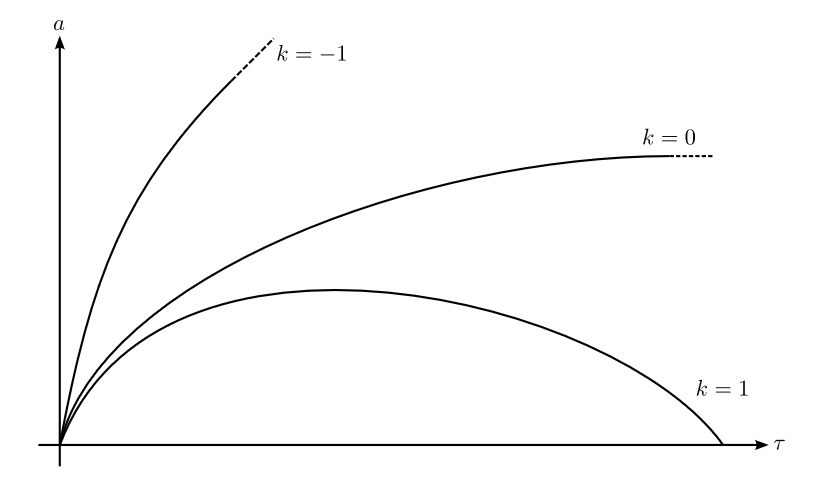
\includegraphics[scale=0.5]{immagini/soluzioni_galassie.png}
        \caption{Soluzioni alle equazioni di Friedmann per le galassie/polveri al variare di $k$.}
        \label{fig.soluzioni_galassie}
    \end{figure}
Le soluzioni corrispondenti a $k=-1,0$ sono tali da comportare un universo in espansione infinita; nel dettaglio si approcciano ad infinito con velocità $\dot{a}= 1, 0$ rispettivamente. La soluzione per $k=1$ invece comporta che l'universo sia in espansione fino a che $a=c$ $(\dot{a}=0)$ per poi contrarsi. Questa soluzione ha portato alla teoria del \textbf{big crunch}.

    \item Radiazione
    \begin{equation*}
        \rho = c a^{-4}
    \end{equation*}
    
    Si ottiene la prima di Friedmann:
    \begin{equation*}
        \dot{a}^2 - \frac{c'}{a^2} + k=0
    \end{equation*}
    dove $c'=\frac{8\pi}{3}$. Le soluzioni sono in tab. \ref{tab.radiazione}.
    \begin{table}
        \centering
        \begin{tabular}{ccc}
        $k=1$ ($S^3$) & $k=0$ ($\mathbb{E}^3$) & $k=-1$ ($H^3$) \\
        \hline
        $a= \sqrt{c'}\left( 1 - (1-\frac{\tau}{\sqrt{c'}})^2\right)^{1/2} $     &  $a= (4c')^{1/4}\tau^{1/2}$ &  $a= \sqrt{c'}\left((1+\frac{\tau}{\sqrt{c'}})^2 -1 \right)^{1/2}$ \\
        \hline
        \end{tabular}
        \caption{Soluzioni per la radiazione.}
        \label{tab.radiazione}
    \end{table}
    \item Energia oscura
    \begin{equation*}
        \rho = \textrm{cost.} = \frac{\Lambda}{8\pi}
    \end{equation*}
    
    La prima di Friedmann:
    \begin{equation*}
        3\frac{\dot{a}^2}{a^2}= \Lambda -3 \frac{k}{a^2}
    \end{equation*}
    ha le soluzioni di tab. \ref{tab.energiaoscura} e fig. \ref{fig.soluzioni_energia}.
    \begin{table}
        \centering
        \begin{tabular}{ccc}
        $k=1$ ($S^3$) & $k=0$ ($\mathbb{E}^3$) & $k=-1$ ($H^3$) \\
        \hline
        $a= \sqrt{\frac{3}{\Lambda}}\cosh \sqrt{\frac{\Lambda}{3}}\tau $     &  $a= e^{ \sqrt{\frac{\Lambda}{3}} \tau}$ &  $a=\sqrt{\frac{3}{\Lambda}}\sinh \sqrt{\frac{\Lambda}{3}}\tau $ \\
        \hline
        \end{tabular}
        \caption{Soluzioni per l'energia oscura.}
        \label{tab.energiaoscura}
    \end{table}
    \begin{figure}
        \centering
        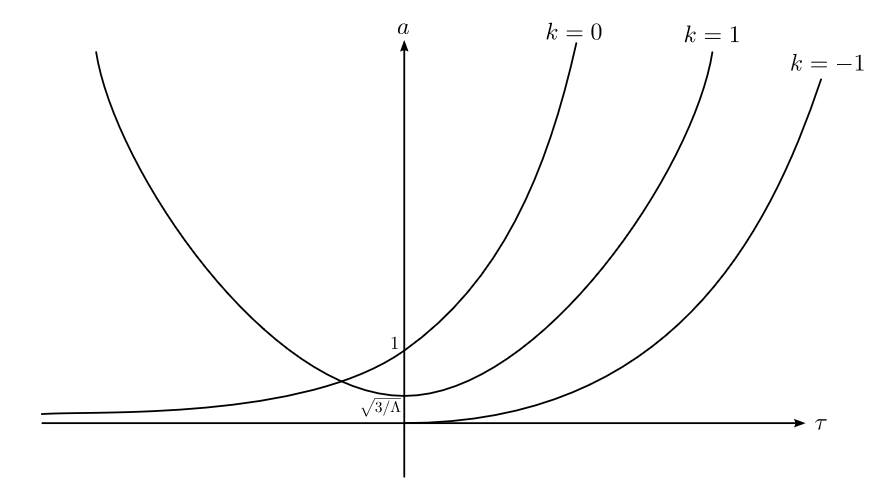
\includegraphics[scale=0.5]{immagini/soluzioni_energia.png}
        \caption{Soluzioni per l'energia oscura al variare di $k$.}
        \label{fig.soluzioni_energia}
    \end{figure}
    In questo caso le soluzioni sono isometriche e descrivono un universo detto \textbf{universo di de Sitter}. Un tale universo è privo di materia ordinaria e con costante cosmologica positiva che determina l'espansione dello stesso.
\end{itemize}

Osserviamo che per $a$ piccolo si ottiene che il termine dominante di $\rho$ è quello dovuto alla radiazione. Questo spiega come negli istanti successivi al big bang, l'universo fosse pervaso dalla radiazione, il cui contributo è andato ad affievolirsi per lasciare spazio ad un'era dominata dalla materia (anzi dall'energia oscura). Il contributo attuale della radiazione è dovuto alla CMB, come radiazione da corpo nero a $2.725$ K .

Al momento la metrica che descrive al meglio il nostro universo è:
\begin{equation}
    ds^2 = - d\tau^2 + e^{ 2\sqrt{\frac{\Lambda}{3}} \tau}( dx^2 + dy^2 + dz^2)
    \label{eq.metrica_universo}
\end{equation}
dove l'espansione dell'universo è esponenziale e lo spazio è a curvatura costante (spazialmente piatto). Un tale universo di de Sitter è detto in \textbf{coordinate inflazionarie}. Con inflazione cosmica si intende quella fase dopo al big bang, avvenuta intorno a $10^{-35} s$ dopo di esso e perdurata per $10^{30} s$, nella quale l'universo ha subito una drastica espansione accelerata, superiore a $10^{30}$ volte. Tale universo primordiale può essere descritto come universo di de Sitter.

Infine riassumiamo la classificazione dei vari spazi: un universo di de Sitter è l'analogo lorentziano ad uno spazio ellittico (la $n-$sfera), mentre un universo anti-de Sitter (corrispondente a $\Lambda <0$) è lo spazio lorentziano corrispondente allo spazio iperbolico. Lo spazio di Minkowski ($\Lambda = 0)$ è evidentemente l'analogo allo spazio euclideo.

\section{Equazioni di Friedmann in forma adimensionale}
Risulta particolarmente utile, soprattutto in ambito applicativo, riscrivere l'equazione di Friedmann (con le costanti esplicitate):
\begin{equation}
    H^2 = \frac{8\pi G}{3 c^2}\rho - \frac{kc^2}{ a^2}
\end{equation}
in termini di quantità adimensionali.  Si definiscono i parametri cosmologici:
\begin{equation}
    \Omega_w = \frac{\rho_{w,0}}{\rho_{crit, 0}}
\end{equation}
dove $w$ è lo stesso introdotto in precedenza e $\rho_{crit,0}$ è la densità critica ottenuta in un universo piatto, $k=0$, alla presente epoca, $H=H_0$:
\begin{equation}
    \rho_{crit,0} = \frac{3c^2}{8\pi G}H_0^2
\end{equation}
Dalla loro definizione, i parametri cosmologici descrivono la frazione di energia della componente $w$ osservata \textit{ad oggi}. 
I parametri sono definiti in modo tale che:
\begin{equation*}
    \sum_w \Omega_w = 1 + \frac{kc^2}{H_0^2}
\end{equation*}
\'E perciò possibile definire il parametro relativo alla curvatura $\Omega_k = - \frac{kc^2}{H_0^2}$. Sulla base di misure delle componenti di materia, radiazione e costante cosmologica nell'Universo, si può determinare il termine di curvatura $k$. Se la densità di energia totale risultasse, come le misure suggeriscono, $\Omega_0 + \Omega_\Lambda \approx 1$ allora l'Universo avrebbe una geometria quasi piatta. \'E bene notare che se $\Omega_k \neq 0$ allora non potrà mai essere veramente nulla e il suo valore evolverà nel tempo; il fatto che ora sia molto prossima a zero, implica che nell'Universo primordiale il suo valore fosse svariati ordini di grandezza ancora più vicina a zero ($o(10^{-16})$ alla nucleosintesi, $o(10^{-60})$ alla fine dell'inflazione). Questo \textit{fine tuning} prende il nome di \textbf{problema della piattezza}. 

L'equazione di Friedmann espressa con i parametri cosmologici diventa:
\begin{equation}
    \left(\frac{H}{H_0}\right)^2 = \frac{\Omega_r}{a^4} + \frac{\Omega_m}{a^3} + \frac{\Omega_k}{a^2} + \Omega_\Lambda
    \label{eq.friedmann_param_cosmologici}
\end{equation}
\section{Redshift cosmologico}
Consideriamo un osservatore, ad esempio una stella, che emette un fotone in $P_1$, il quale viene ricevuto da un secondo osservatore nel punto $P_2$ in un tempo proprio $\tau=\tau_2$. I punti $P_1, P_2$ sono punti delle ipersuperfici di omogeneità $\Sigma_\tau$ con $\tau = \tau_1, \tau_2$. Chiamiamo $u_i$ il relativo vettore ortogonale alla superficie e $\omega_i$ la frequenza emessa o ricevuta.
\begin{figure}
    \centering
    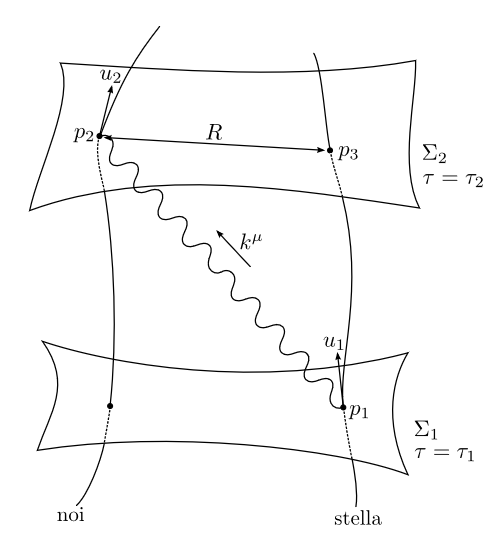
\includegraphics[scale=0.6]{immagini/redshiftcosmo.png}
    \caption{Redshift cosmologico}
    \label{fig.redshiftcosmo}
\end{figure}
Detto $k^\mu$ il vettore d'onda della luce, si avrà:
\begin{align*}
    \omega_1 = -k_\mu u_1^\mu && \omega_2 = - k_\mu u_2^\mu
\end{align*}

Vale in generale che si può trovare un vettore di Killing $\xi^\mu$ che punta nella direzione della proiezione di $k_\mu$ su $\Sigma_{\tau_1}$ in $P_1$, e similmente per $P_2$\footnote{Ad esempio per $k=0$, $\Sigma$ è piatta e possiamo assumere che $k_\mu$ proiettato su $\Sigma_{\tau_1}$ in $P_1$ sia nella direzione $\partial_x$ (altrimenti eseguiamo rotazione). Vale $<k,\partial_y> = < k, \partial_z> = 0$ al tempo iniziale; poiché $\partial_y, \partial_z$ sono di Killing e $k$ è tangente alla geodetica, questi prodotti scalari si conservano e rimangono tali lungo essa fino in $P_2$. Pertanto la proiezione di $k_\mu$ su $\Sigma_{\tau_2}$ in $P_2$ rimane lungo $\partial_x$ e $\xi =\partial_x$ è il vettore di Killing in questione. Ragionamento simile per $k=\pm 1$.}.

Inoltre dalla metrica, $ds^2 =  a^2(\tau)d\Omega^2$, si ha:
\begin{equation*}
    \frac{<\xi , \xi>^{1/2}|_{P_1}}{<\xi , \xi>^{1/2}|_{P_2}} = \frac{a(\tau_1)}{a(\tau_2)}
\end{equation*}
Scomponendo il vettore d'onda nelle componenti parallele e ortogonali all'ipersuperficie per il motivo prima detto:
\begin{equation*}
    k_\mu = A u_\mu + B \frac{\xi_\mu}{(\xi^2)^{1/2}}
\end{equation*}
dunque per la condizione $k_\mu k^\mu=0$ si avrà $A=B$ e dunque:
\begin{equation*}
    0 = A\left(  u_\mu k^\mu + \frac{\xi_\mu k^\mu}{(\xi^2)^{1/2}}\right) \iff - u_\mu k^\mu =  \frac{\xi_\mu k^\mu}{(\xi^2)^{1/2}}
\end{equation*}
ottenendo dunque:
\begin{equation*}
    \omega_{1,2} = \frac{\xi_\mu k^\mu}{(\xi^2)^{1/2}} \Big|_{P_{1,2}}
\end{equation*}

Facendo il rapporto si ottiene la relazione del \textbf{redshift cosmologico}:
\begin{equation}
    \frac{\omega_2}{\omega_1} =    \frac{<\xi , \xi>^{1/2}|_{P_1}}{<\xi , \xi>^{1/2}|_{P_2}} = \frac{a(\tau_1)}{a(\tau_2)}
    \label{eq.redshift_formale}
\end{equation}
dovuto all'espansione dell'universo, per la quale $a(\tau_1) \neq a(\tau_2)$.

Immaginiamo di essere l'osservatore $P_2$ e per convenienza richiamiamo $\tau_2 \rightarrow \tau_0$ ad indicare l'attuale tempo di osservazione, mentre $\tau_1 \rightarrow \tau_{em}$ per indicare quello di emissione del segnale, così siamo in una notazione più familiare. Utilizzando la convenzione usata in cosmologia dove il fattore di scala ad oggi è $a(\tau_0) = 1$, l'eq. \ref{eq.redshift_formale} diventa $\omega_{em}/\omega_{0} = a^{-1}(\tau_{em})$. Il redshift $z$ è definito:
\begin{equation}
    z = \frac{\omega_{em} - \omega_0}{\omega_0}
    \label{eq.redshift_z}
\end{equation}
e quindi si ottiene la relazione tra il fattore di scala e il redshift:
\begin{equation}
    a = (1+z)^{-1}
    \label{eq.redshift_relazione_a_z}
\end{equation}

Se differenziamo la formula del redshift $1+z = a(t_0)/a(t_{em})$, rispetto il tempo di osservazione $t_0$:
\begin{equation*}
    \frac{dz}{dt_0} = \frac{\Dot{a}(\tau_0)}{a(\tau_{em})} - \frac{a(\tau_0) \Dot{a(\tau_{em})}}{a^2(\tau_{em})}\frac{d\tau_{em}}{d\tau_0} = \left[H_0 - H(\tau_{em})\frac{d\tau_{em}}{d\tau_0} \right](1+z)
\end{equation*}
e richiamiamo il fatto che $\frac{d\tau_{em}}{d\tau_0} = \frac{1}{1+z}$ per gli stessi argomenti usati poco fa per definire il redshift, otteniamo:
\begin{equation*}
    \frac{dz}{d\tau_0} = H_0(1+z) - H(\tau_{em})
\end{equation*}
Con questa formula è possibile determinare la variazione del redshift col tempo o, viceversa, il valore del rate di espansione al tempo di emissione.
\section{Distanza di luminosità e diametro-angolare}
Per distanze cosmologiche dire che \virgolette{un oggetto è distante \textit{tot} anni-luce da noi} non è ben definito a meno di non fornire una definizione chiara del tipo di misura di distanza che si è effettuata. In particolar modo le misure di distanza che possiamo fare osservando il cielo sono legate al flusso di luce che ci giunge e alle dimensioni angolari degli oggetti.

Per quanto riguarda l'universo locale o semplicemente per nostra esperienza nella vita di tutti i giorni, oggetti con pari luminosità (intrinseche) posti a distanze differenti verranno osservati con luminosità (apparenti) diverse, minore per quello più distante. In uno spazio euclideo, la radiazione luminosa viene emessa isotropicamente e misurata con un flusso che scala con la superficie sferica di raggio pari alla distanza di osservazione $d$ secondo:
\begin{equation*}
    \Phi = \frac{L}{4\pi d^2}
\end{equation*}
Ovviamente una formula del genere è soggetta a possibili correzioni dovute all'assorbimento interstellare e/o intergalattico, che tuttavia trascuriamo ai nostri fini.
La quantità $L$ è la luminosità intrinseca dell'oggetto; tale valore può essere determinato per altre vie ad esempio utilizzando le cosiddette \emph{candele standard}, ovvero corpi per i quali possiamo risalire alla loro energia emessa in unità di tempo, dopo aver analizzato fenomeni \virgolette{standard} che avvengono all'interno di essi; sono un esempio le Cefeidi, stelle che variano le loro dimensioni con periodo proporzionale alla loro luminosità intrinseca, oppure le già citate supernove tipo 1A le quali posseggono una luminosità di picco comune al momento dell'esplosione.

Risulta abbastanza chiaro che quando si parla di distanze cosmologiche, dove i parametri cosmologici ed in particolare la geometria dello spaziotempo diventano rilevanti, tale formula deve essere cambiata. Determiniamo dunque la corretta formula nella cosmologia di FLRW.

Riscriviamo la metrica FLRW nella forma:
\begin{equation}
    ds^2 = -d\tau^2 +\left[ d\psi^2 + S_k(\psi)^2(d\theta^2 + \sin\theta^2 d\phi^2) \right]
    \label{eq.metrica_flrw_esplicitata}
\end{equation}
con
\begin{equation*}
    S_k(\psi) = \left\{ \begin{array}{cc}
        \sin\psi      & k= 1 \\
        \psi   & k= 0 \\
        \sinh\psi & k = -1 
    \end{array}\right.
\end{equation*}
Come conseguenza una sfera $S^2$ possiede ora una superficie di area $4\pi S_k^2(\psi)$. L'altro effetto da tenere in considerazione è quanto determinato nel paragrafo precedente ovvero il redshift delle luce dovuto alla distanza cosmologica. Un fotone emesso a frequenza $\nu_1$ giungerà all'osservatore con la frequenza (e quindi energia secondo l'equazione di Einstein-Planck):
\begin{equation*}
    \nu_0 = \frac{\nu_1}{1+z} \implies E_0 = \frac{E_1}{1+z}
\end{equation*}
dove $z$ è il redshift.
Con queste semplici considerazioni otteniamo che il flusso osservato ad una distanza comovente $\psi$ è:
\begin{equation}
    \Phi = \frac{L}{4\pi S_k(\psi)^2(1+z)^2}
    \label{eq.flusso_dist_cosmologica}
\end{equation}
Questo ci porta a definire la \textbf{distanza di luminosità}:
\begin{equation}
    d_L(\psi) =S_k(\psi)(1+z)
    \label{eq.luminosity_distance}
\end{equation}
Confrontando le due luminosità $L, \phi$ allora si ottiene che $d_L$ è una quantità effettivamente misurabile. Essa permette proprio la conversione tra luminosità intrinseca e apparente. Le tipiche distanze date in \virgolette{anni-luce} sono corrispondenti a $d_L$ che è monotona crescente con $z$.


Passando alla misura delle dimensioni angolari, come verrà mostrato, ci saranno importanti differenze rispetto il caso euclideo. La lunghezza d'arco $l$ di un oggetto è ottenuta dalla metrica FLRW di eq. \ref{eq.metrica_flrw_esplicitata} considerando $d\psi = d\phi =0$ a tempo fissato e integrando sull'angolo osservato:
\begin{equation*}
    l = \int ds = \int a(\tau_e)S_k(\psi)d\theta = a(\tau_e)S_k(\psi)\alpha
\end{equation*}
dove $\alpha$ è proprio l'angolo di estensione dell'oggetto; $\tau_e$ è il tempo di emissione del segnale e la relazione del redshift lega $a^{-1}(\tau_e) = 1+ z$. La \textbf{distanza diametro-angolare} è data dal rapporto tra la lunghezza d'arco $l$ e il rispettivo angolo $\alpha$ ed è pertanto:
\begin{equation}
    d_A(\psi) = \frac{S_k(\psi)}{1+z}
    \label{eq.distanza_diametro_angolare}
\end{equation}
Il suo utilizzo è quindi quello di convertire angoli in lunghezze fisiche trasverse $l = \alpha d_A$. In fig. \ref{fig.distanza_diametro_angolare_modelli} è mostrato come varia $d_A$ per alcuni modelli cosmologici. Si può notare che ad alto redshift $z>1$ le dimensioni angolari di un oggetto a $l=\cost$ aumentano invece che diminuire. Si potrebbe pensare che ciò porti al cosiddetto \textit{confusion limit} ovvero al fatto che gli oggetti cosmologici troppo lontani siano così grandi da sovrapporsi. Tuttavia questo non si verifica poiché le galassie ad alto redshift sono galassie giovani e quindi intrinsecamente piccole.
Si può anche notare che per determinati valori di $d_A$ vi corrispondono due ben differenti valori di $z$; questo corrisponde ad avere galassie con le stesse dimensioni angolari, ma di epoche e distanze ben differenti.
\begin{figure}[b]
    \centering
    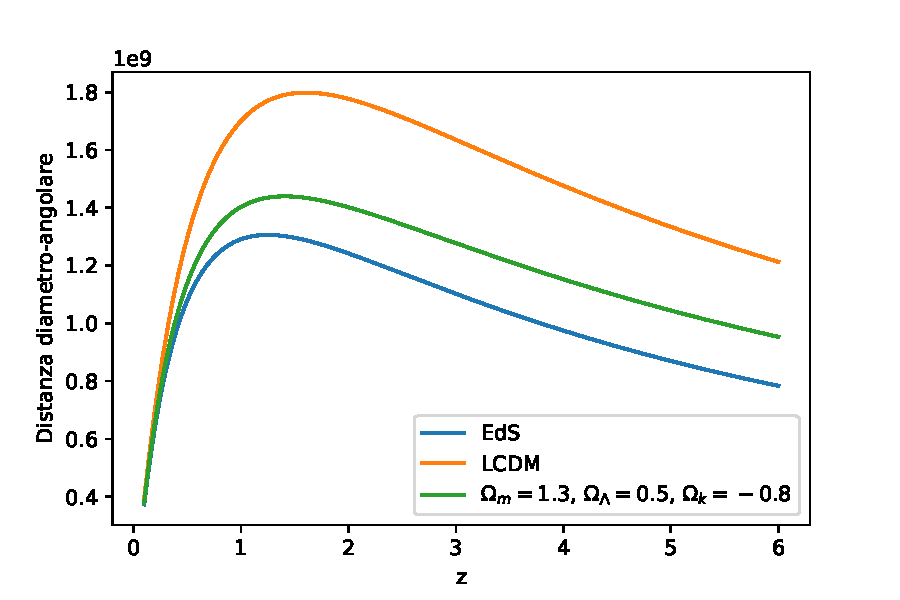
\includegraphics[scale=0.7]{immagini/distanza_diametro_angolare.pdf}
    \caption{Distanza diametro-angolare di eq. \ref{eq.distanza_diametro_angolare} in funzione del redshift $z$ in differenti modelli cosmologici. Einstein-de Sitter ($\Omega_m =1$), LCDM ($\Omega_m=0.3$, $\Omega_\Lambda = 0.7$, $\Omega_k= 0$) e un modello di materia chiuso. Si è usato $H_0 = 68 $ km/(Mpc s).}
    \label{fig.distanza_diametro_angolare_modelli}
\end{figure}

Se una sorgente luminosa ha una luminosità intrinseca per unità di area propria $\mathcal{L}$ allora per quanto visto, la sua luminosità apparente per una patch di area $A$ sarà $l = \mathcal L A/4\pi d_L^2$ e l'angolo solido sotteso da questa patch sarà $\Omega = A/d_A^2$. Pertanto si definisce la \textbf{brillanza superficiale} come la luminosità apparente per angolo solido:
\begin{equation}
    B = \frac{l}{\Omega} = \frac{\mathcal L d_A^2}{4\pi d_L^2} = (1+z)^{-4}\left( \frac{\mathcal L}{4\pi}\right)
    \label{eq.brillanza_superficiale}
\end{equation}
La quantità $(1+z)^{-4}$ è chiamata \textbf{cosmological dimming} ed è responsabile delle difficoltà legate all'osservazione ad alto redshift. La brillanza superficiale è stata utilizzata per verificare sperimentalmente che il fenomeno di redshift cosmologico fosse dovuto all'espansione dell'Universo e non a fenomeni di \textit{tired light}. Teorie di questo tipo prevedono l'Universo come statico e che i fotoni perdano la loro energia tramite meccanismi di differente natura. L'indipendenza tuttavia dalla misura diametro-angolare rende possibile l'esclusione di queste teorie per mezzo del test della brillanza superficiale. 